\subsubsection{Gaussian Mixture Models}
\label{sec:GMM}
One of the most common distributions is the Gaussian distribution $ \mathcal{N}(\mu,\sigma)$. Sometimes this model is not quiet enough to capture the underlying distribution. In such cases can a mixture of Gaussian distributions be created to fit a underlying distribution. This principal is shown in figure \ref{fig:mixturemodel}. 

\begin{figure}[H]
\centering
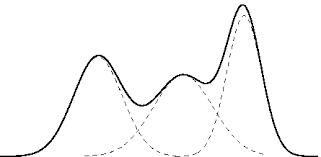
\includegraphics[scale=0.5]{billeder/MixtureModel}
\caption{Gaussian Mixture Model Principe}
\label{fig:mixturemodel}
\end{figure}

This method can be generalized up in a multidimensional space, to fit the feature space. In a multidimensional model we introduce the covariance matrix $\Sigma$ that like $\sigma$ gives the deviation of a Gaussian model. The Gaussian mixture model can therefore be described as: 

\begin{equation}
 P(x) = \sum\limits_{k=1}^K{ \Pi_k \mathcal{N}(x|\mu_k,\sigma_k) }
\label{eq:mixturemodel}
\end{equation}

Where $\Pi_k$ is a weight called the mixture parameter, that is used to differentiate the individual Gaussian distributions in the model. knowing this we can also describe the mixture model from equation \ref{eq:mixturemodel} as: 

\begin{equation}
 P(x) = \sum\limits_{k=1}^K{ P(k) P(x|k) }
\label{Eq:mixturemodel}
\end{equation}

In order to use a the mixture model, the different distributions must first be found. This topic will be discussed in section \ref{sec:k-means} and \ref{sec:EMAlgorithm}

\subsubsection{k-means Algorithm}
\label{sec:k-means}

One way of finding groupings of data, in the feature space, is by using the k-means algorithms. This algorithm tries to split the data in k groups. This is done by following 4 three step iterating proses. 

\begin{enumerate}
  \item Initialize means: Select k random mean values in the feature set. 
  \item Assign responsibility: For each point, find the closest mean points and make it responsible for that point.
  \label{step:iteratemeans} 
  \item Calculate new mean: Move each mean point to the mean value of the cluster of points the mean is responsible for. 
  \item Continue whit step \ref{step:iteratemeans}, till no change in points. 
\end{enumerate}

On figure \ref{fig:kmeans} is illustrated how the k-means in 6 iterations split the data up in 3 clusters.

\begin{figure}[H]
\centering
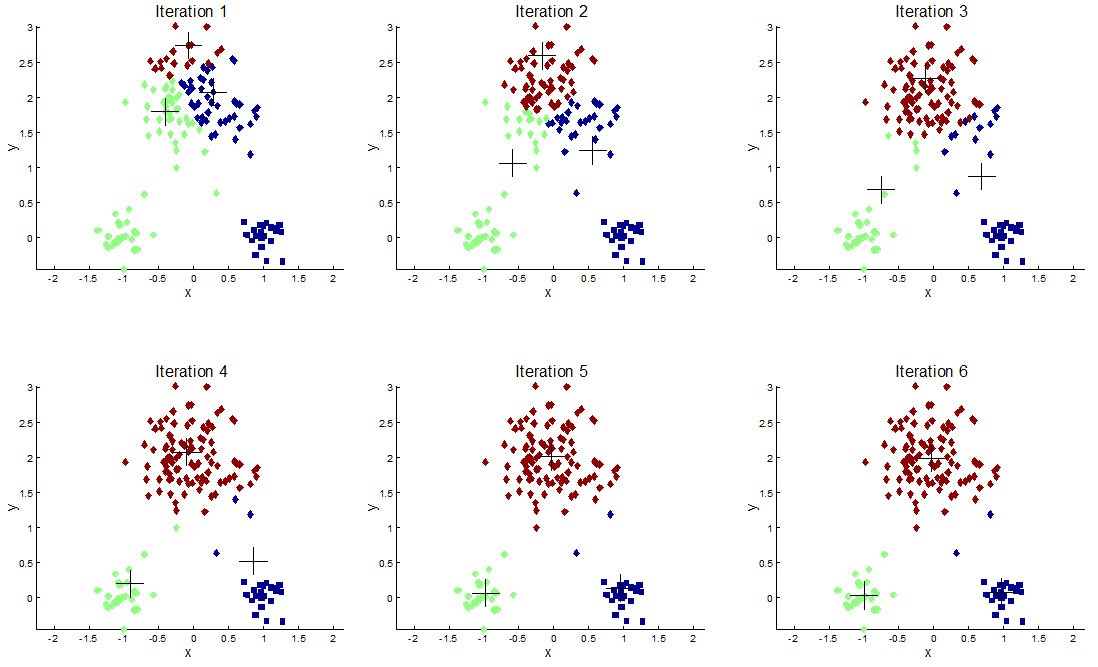
\includegraphics[scale=0.6]{billeder/kmeansclustering}
\caption{K-means used on a data set}
\label{fig:kmeans}
\end{figure}

The result of this process will differ depending on the initial mean guesses. This is especially the case is there is no natural groupings in the dataset. In this case the algorithm will still split up the data in k clusters there are side by side. This is illustrated on figure \ref{fig:badkmeans}, where the k-means algorithm tries to cluster points, distributed uniformly on a circle, in 7 clusters. 

\begin{figure}[H]
\centering
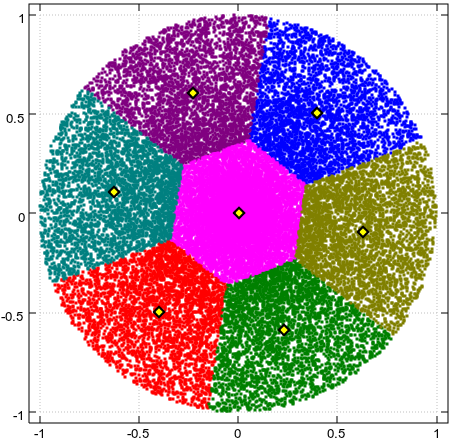
\includegraphics[scale=0.5]{billeder/CircleClusters}
\caption{K-means used on points distributed uniformly on a circle}
\label{fig:badkmeans}
\end{figure}

\subsubsection{EM Algorithm For Gaussian Mixture Models}
\label{sec:EMAlgorithm}

As discussed in section \ref{sec:GMM} it is important to have a method of finding the best Gaussian distributions in the data set to create a good mixture model. The best Gaussian Mixture Models that fits the data can be described as optimising equation \ref{eq:maxgmm}.

\begin{equation}
 L(x) = \sum\limits_{n=1}^N{\log{\sum\limits_{k}^K P(k) P(\textbf{x}_n|k) }}
\label{eq:maxgmm}
\end{equation}

To find the maximum of equation \ref{eq:maxgmm}, we find the differentiated and set et equal zero. 

 \begin{equation}
 \frac{\partial L(\textbf{x})}{\partial{\mathbold{\mu}_k}} = 0
\label{eq:partialzero}
\end{equation}

From equation \ref{eq:mixturemodel} and \ref{eq:partialzero} the following optimisations equations can be found: 

\begin{equation}
 N_k = \sum\limits_{k}^K P(k|\textbf{x}_n)
 \label{eq:em1}
\end{equation}
\begin{equation}
 P(k)= \Pi_k = \frac{N_k}{N}
 \label{eq:em2}
\end{equation}
\begin{equation}
 \mathbold{\Sigma}_k= \frac{1}{N_k} \sum\limits_{n}^N{ P(k|\textbf{x}_n) (\textbf{x}_n -\mathbold{\mu}_n)(\textbf{x}_n-\mathbold{\mu}_k)^\intercal}
 \label{eq:em3}
\end{equation}
\begin{equation}
 \mathbold{\mu}_k= \frac{1}{N_k} \sum\limits_{n}^N{ P(k|\mathbold{x}_n) \mathbold{x}_n}
 \label{eq:em4}
\end{equation}

The variable $N_k$ can be seen as the effective number of samples in a cluster, and $N$ is the total number of samples. The $P(k|x_n)$ term can be seen as the responsibility a center point has for that point. Unlike the K-means algorithm the all center points are responsible for all points, but the level of responsibility is different from center point to center point. To find the optimal center points $\mu_k$, and there deviations $\Sigma_k$ the EM algorithm can be used. This is based on a the idea of a E-step, called the estimation step, and a M-step called the maximisation step. Much like the k-means does this also have 4 iterative steps. 


\begin{enumerate}
  \item Initialize Parameters: Select k random values for $\mu_k$ , $\Sigma_k$ , $\Pi_k$
  \item E-Step: Update the responsibility by using Bayes' theorem stating: 
 \begin{equation}
 	P(k|x) = \frac{P(x|k) P(k)}{P(x)} = \frac{P(x|k) P(k)}{\sum\limits_{k}^K{ P(x|k) P(k)}}
 \end{equation}
  
  \item M-Step: Maximize the Gaussian mixture model parameters by using equations \ref{eq:em1}, \ref{eq:em2}, \ref{eq:em3} and \ref{eq:em4}. 
  
  \item Continue whit step 2, till no change in Gaussian mixture model parameters. 
\end{enumerate}

Like the k-means algorithm does this algorithm also map a predetermined number of Gaussian distributions to the dataset. The optimal amount must be found though exploration. On figure \ref{fig:UGMM} we see how the EM algorithm has been used to map 3 Gaussian mixture model to a dataset. 

\begin{figure}[H]
\centering
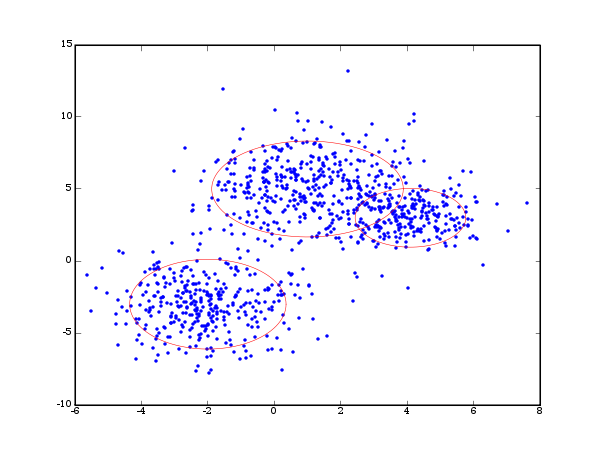
\includegraphics[scale=0.5]{billeder/UGMM}
\caption{EM Algorithm Used On Data To Create GMM}
\label{fig:UGMM}
\end{figure}

Like for the k-means the initial start estimates for the mean value is important for a good result, and a fast execution time. A normal approach is to use the k-means algorithm first, and use the final means as the start estimate in the em algorithm. In order to reduce the training time, the model is sometimes reduced in complicity. Instead of a full Gaussian distribution a spherical covariance or a completely diagonal covariance is used. 

\subsubsection{Unsupervised Gaussian Mixture Model}
\label{sec:UGMM}
Sometimes the training data is unlabelled, which mean that the classes is unknown. In such data there can still be some underlying structures, that can be used to classify the data. The goal of unsupervised learning is to discover these structures, and create the classes from them. \\ \ \\
One approach of this is to select a number of desired classes, and try finding clusters in the data to fit to the classes. This can be done whit the k-means as shown in figure \ref{fig:kmeans}.  where 3 classes is found to fit the data. Likewise can the Gaussian mixture model also be used to find distributions that describes the classes. This can be seen in figure \ref{fig:UGMM} where 3 Gaussian distributions is fit to the unlabelled data. \\ \ \\

In the speech recognition case we have investigated if it is possible to use the Gaussian mixture model as a unsupervised method to find the 3 persons: Nicolai, Rasmus and Rune. For this to work the features must be placed in separated clusters corresponding to the persons. 

When evaluating this we see that the classes found does not correspond to the 3 know classes. The when looking at the errors on table \ref{tab:resultTableUGMM}, it is seen how the error for every one over 50%. 


\begin{table}[H]
\centering
\begin{tabular}{ll}
\hline
Total Error   & 65.24 \% \\ \hline
Nicolai Error & 53.10 \% \\
Rasmus Error  & 78.34 \% \\
Rune Error    & 64.27 \% \\ \hline
\end{tabular}
\caption{Unsupervised GMM Results}
\label{tab:resultTableUGMM}
\end{table}
 
This means that this method is not able to automatically split the data up in the desired classes.
 
\subsubsection{Supervised Gaussian mixture model}
\label{sec:EMGMM}

What if we used the same method to train the data, but in a supervised manner. A other method is to train a Gaussian mixture model for each class, and use this to classify. A Gaussian mixture model was trained to each voices. To find the optimal amount of Gaussian distributions for each model, a experiment was done where we started at one Gaussian distribution per model and ended whit 10.

\begin{figure}[H]
\centering
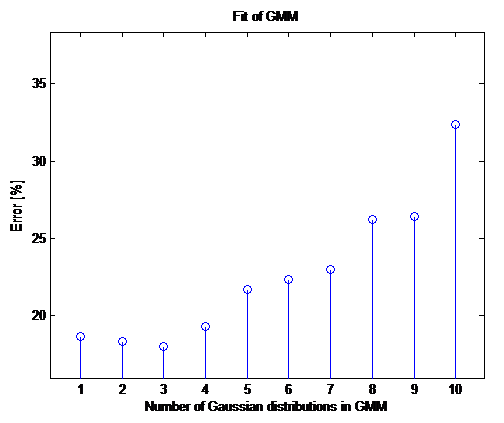
\includegraphics[scale=0.7]{billeder/fitGmm}
\caption{GMM fit in relation to number of Gaussian distributions}
\label{fig:fitGMM}
\end{figure}

As seen on figure \ref{fig:fitGMM}, three Gaussian distributions in each GMM is the one that gives the lowest error. To ensure that 18\% is the best we can achieve whit this model, the model is retrained whit random initializations. The best fit found to be 15.64 \% error. This can be calculated from the confusion matrix seen in figure \ref{fig:conmatGMM}. 

\begin{figure}[H]
\centering
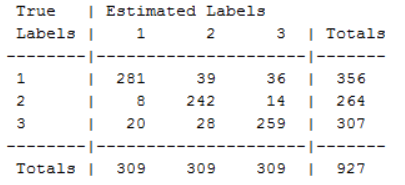
\includegraphics[scale=0.7]{billeder/conmatgmm}
\caption{Confusion matrix for supervised Gaussian mixture model }
\label{fig:fitGMM}
\end{figure}

Here it is seen how this model is relative good at separating the data in the  the three classes. This model have the most trouble finding Rasmus, this is noticeable different from the other models where Rune is the hardest to recognize. 

%------------------------------------------------